% simple.tex - A simple article to illustrate document structure.

% Arshad Ansari

\documentclass[12pt]{book}
\usepackage[T1]{fontenc}
\usepackage[utf8]{inputenc}
\usepackage{anyfontsize}
\usepackage{mathptmx}
\usepackage{graphicx}
\usepackage[margin=1in]{geometry}
\usepackage{mdwlist}
\usepackage{longtable}
\graphicspath{ {figures/} }


\begin{document}

% Front Cover page
\thispagestyle{empty}

\begin{center}
	\fontsize{14}{30}\selectfont \textbf{A\\SPECIAL TOPIC SEMINAR\\ On}\\
  	\fontsize{20}{30}\selectfont \textbf{Text Classification Techniques}\\
  	\fontsize{14}{24}\selectfont Submitted in partial fulfillment of the requirement of Universirty of Mumbai\\For the Degree of\\
  	\fontsize{16}{30}\selectfont \textbf{Master of Engineering}\\
  	\fontsize{14}{30}\selectfont \textbf{Information Technology (AI and Robotics)} \\
  	by\\
  	\textbf{Mr. Mohammed Arshad Ansari}\\
  	\textbf{Registeration No: XYZ,}\\
  	Supervisor\\
  	\textbf{Prof. Sharvari Govilkar}\\
	\vspace{30mm}
	\begin{figure}[ht!]
	  \centering
	  
\includegraphics[width=30mm]{piit.png}
	\end{figure}
  	\fontsize{14}{20}\selectfont \textbf{DEPARTMENT OF INFORMATION TECHNOLOGY\\PILLAI'S INSTITUTE OF INFORMATION TECHNOLOGY,\\
	ENGINEERING, MEDIA STUDIES \& RESEARCH\\ NEW PANVEL - 410206\\UNIVERSITY OF MUMBAI\\Academic Year 2014-15}

\end{center}

% Certificate page
\begin{figure}[ht!]
    \centering
    
\includegraphics[width=30mm]{piit.png}
\end{figure}
\begin{center}
    \fontsize{14}{20}\selectfont \textbf{PILLAI'S INSTITUTE OF INFORMATION TECHNOLOGY,\\ENGINEERING, MEDIA STUDIES \& RESEARCH\\ NEW PANVEL}\\
    \fontsize{22}{50}\selectfont \textbf{\underline{CERTIFICATE}}\\
    \fontsize{14}{40}\selectfont \textit{This is to certify that}\\
    \fontsize{14}{40}\selectfont \textbf{Mr. Mohammed Arshad Ansari}\\
    \fontsize{14}{40}\selectfont \textit{have satisfactorily completed the requirements of the Special Topic Seminar entitled}\\
    \fontsize{14}{40}\selectfont \textbf{On}\\
    \fontsize{20}{40}\selectfont \textbf{TEXT CLASSIFICATION TECHNIQUES}\\
    \fontsize{14}{40}\selectfont \textit{as prescribed by the \textbf{University of Mumbai}, under the guidance of \textbf{Prof. Sharvari Govilkar}}\\
    \vspace{30mm}
    \noindent --------------------------\hfill--------------------------\\
    \noindent Project Guide \hfill HOD\\
    \noindent\hfill \fontsize{14}{20}\selectfont Department of Information Technology


\end{center}
	

% Acknowledgement page
\begin{center}

    \fontsize{14}{60}\selectfont \textbf{Acknowledgement}\\
    \vspace{5mm}
    \fontsize{12}{20}\selectfont This is the greatest acknowledgement ever written. It was written to acknowledge that which is always acknowledged, but never really means any thing. I am sure a lot of people will acknowlege that which is written in the acknowledgement.\\

    \vspace{5mm}
    \fontsize{12}{20}\selectfont This is the greatest acknowledgement ever written. It was written to acknowledge that which is always acknowledged, but never really means any thing. I am sure a lot of people will acknowlege that which is written in the acknowledgement.\\

    \vspace{5mm}
    \fontsize{12}{20}\selectfont This is the greatest acknowledgement ever written. It was written to acknowledge that which is always acknowledged, but never really means any thing. I am sure a lot of people will acknowlege that which is written in the acknowledgement.\\
    
    \vspace{60mm}
    \noindent\hfill \fontsize{14}{20}\selectfont -----------------------------\\
    \noindent\hfill \fontsize{14}{20}\selectfont Mohammed Arshad Ansari
\end{center}

\tableofcontents


\addcontentsline{toc}{chapter}{i. List of Figures}
\listoffigures

\addcontentsline{toc}{chapter}{ii. List of Tables}
\listoftables

\clearpage

\pagenumbering{arabic}

\chapter{Introduction}

Text classification or Document classification is a problem in library science, information science and computer science. The task is to assign a document to one or more classes or categories. This may be done "manually" (or "intellectually") or algorithmically. The intellectual classification of documents has mostly been the province of library science, while the algorithmic classification of documents is used mainly in information science and computer science. The problems are overlapping, however, and there is therefore also interdisciplinary research on document classification.

The documents to be classified may be texts, images, music, etc. Each kind of document possesses its special classification problems. When not otherwise specified, text classification is implied.

Documents may be classified according to their subjects or according to other attributes (such as document type, author, printing year etc.). In the rest of this article only subject classification is considered. There are two main philosophies of subject classification of documents: The content based approach and the request based approach. \cite{wikipedia-textclassification}

\section{Types of classification}
Content based classification is classification in which the weight given to particular subjects in a document determines the class to which the document is assigned. It is, for example, a rule in much library classification that at least 20\% of the content of a book should be about the class to which the book is assigned.In automatic classification it could be the number of times given words appears in a document.

Request oriented classification (or -indexing) is classification in which the anticipated request from users is influencing how documents are being classified. The classifier asks himself: “Under which descriptors should this entity be found?” and “think of all the possible queries and decide for which ones the entity at hand is relevant” (Soergel, 1985, p. 230[2]).

Request oriented classification may be classification that is targeted towards a particular audience or user group. For example, a library or a database for feminist studies may classify/index documents differently when compared to a historical library. It is probably better, however, to understand request oriented classification as policy based classification: The classification is done according to some ideals and reflects the purpose of the library or database doing the classification. In this way it is not necessarily a kind of classification or indexing based on user studies. Only if empirical data about use or users are applied should request oriented classification be regarded as a user-based approach.

\textbf{Automatic document classification} tasks can be divided into three sorts: \\
\begin{itemize*}
  \item \textbf{\textit{Supervised document classification}}; where some external mechanism (such as human feedback) provides information on the correct classification for documents, \\
  \item \textbf{\textit{Unsupervised document classification}}; (also known as document clustering), where the classification must be done entirely without reference to external information, and \\
  \item \textbf{\textit{Semi-supervised document classification}}: where parts of the documents are labeled by the external mechanism.
\end{itemize*}


\section{Techniques for classification}


\begin{enumerate*}
  \item \textbf{\textit {Expectation maximization (EM)}}: The EM algorithm proceeds from the observation that the following is a way to solve these two sets of equations numerically. One can simply pick arbitrary values for one of the two sets of unknowns, use them to estimate the second set, then use these new values to find a better estimate of the first set, and then keep alternating between the two until the resulting values both converge to fixed points. It's not obvious that this will work at all, but in fact it can be proven that in this particular context it does, and that the derivative of the likelihood is (arbitrarily close to) zero at that point, which in turn means that the point is either a maximum or a saddle point.
  \item \textbf{\textit {Naive Bayes classifier}}: In simple terms, a naive Bayes classifier assumes that the value of a particular feature is unrelated to the presence or absence of any other feature, given the class variable. For example, a fruit may be considered to be an apple if it is red, round, and about 3" in diameter. A naive Bayes classifier considers each of these features to contribute independently to the probability that this fruit is an apple, regardless of the presence or absence of the other features.\\For some types of probability models, naive Bayes classifiers can be trained very efficiently in a supervised learning setting. In many practical applications, parameter estimation for naive Bayes models uses the method of maximum likelihood; in other words, one can work with the naive Bayes model without accepting Bayesian probability or using any Bayesian methods.
  \item \textbf{\textit {tf–idf}}:  is a numerical statistic that is intended to reflect how important a word is to a document in a collection or corpus.[1]:8 It is often used as a weighting factor in information retrieval and text mining. The tf-idf value increases proportionally to the number of times a word appears in the document, but is offset by the frequency of the word in the corpus, which helps to control for the fact that some words are generally more common than others.\\ Variations of the tf–idf weighting scheme are often used by search engines as a central tool in scoring and ranking a document's relevance given a user query. tf–idf can be successfully used for stop-words filtering in various subject fields including text summarization and classification.
  \item \textbf{\textit {Latent semantic indexing}}: is an indexing and retrieval method that uses a mathematical technique called singular value decomposition (SVD) to identify patterns in the relationships between the terms and concepts contained in an unstructured collection of text. LSI is based on the principle that words that are used in the same contexts tend to have similar meanings. A key feature of LSI is its ability to extract the conceptual content of a body of text by establishing associations between those terms that occur in similar contexts.
  \item \textbf{\textit {Support vector machines (SVM)}}: is  supervised learning models with associated learning algorithms that analyze data and recognize patterns, used for classification and regression analysis. Given a set of training examples, each marked as belonging to one of two categories, an SVM training algorithm builds a model that assigns new examples into one category or the other, making it a non-probabilistic binary linear classifier. An SVM model is a representation of the examples as points in space, mapped so that the examples of the separate categories are divided by a clear gap that is as wide as possible. New examples are then mapped into that same space and predicted to belong to a category based on which side of the gap they fall on.
  \item \textbf{\textit {Artificial neural network}}: are computational models inspired by an animal's central nervous systems (in particular the brain), and are used to estimate or approximate functions that can depend on a large number of inputs and are generally unknown. Artificial neural networks are generally presented as systems of interconnected "neurons" which can compute values from inputs, and are capable of learning thanks to their adaptive nature.
  \item \textbf{\textit {K-nearest neighbour algorithms}}:  is a non-parametric method used for classification and regression.[1] In both cases, the input consists of the k closest training examples in the feature space. The output depends on whether k-NN is used for classification or regression:
	\begin{itemize*}
	  \item In k-NN classification, the output is a class membership. An object is classified by a majority vote of its neighbors, with the object being assigned to the class most common among its k nearest neighbors (k is a positive integer, typically small). If k = 1, then the object is simply assigned to the class of that single nearest neighbor.
	  \item In k-NN regression, the output is the property value for the object. This value is the average of the values of its k nearest neighbors.
	\end{itemize*}
  \item \textbf{\textit {Decision trees such as ID3 or C4.5}}: uses a decision tree as a predictive model which maps observations about an item to conclusions about the item's target value. It is one of the predictive modelling approaches used in statistics, data mining and machine learning. More descriptive names for such tree models are classification trees or regression trees. In these tree structures, leaves represent class labels and branches represent conjunctions of features that lead to those class labels.
  \item \textbf{\textit {Concept Mining}}:  is an activity that results in the extraction of concepts from artifacts. Solutions to the task typically involve aspects of artificial intelligence and statistics, such as data mining and text mining.[1] Because artifacts are typically a loosely structured sequence of words and other symbols (rather than concepts), the problem is nontrivial, but it can provide powerful insights into the meaning, provenance and similarity of documents.
  \item \textbf{\textit {Multiple-instance learning}}: is a variation on supervised learning. Instead of receiving a set of instances which are individually labeled, the learner receives a set of labeled bags, each containing many instances. In the simple case of multiple-instance binary classification, a bag may be labeled negative if all the instances in it are negative. On the other hand, a bag is labeled positive if there is at least one instance in it which is positive. From a collection of labeled bags, the learner tries to either (i) induce a concept that will label individual instances correctly or (ii) learn how to label bags without inducing the concept.
  \item \textbf{\textit {Natural language processing approaches}}:  is a field of computer science, artificial intelligence, and linguistics concerned with the interactions between computers and human (natural) languages. As such, NLP is related to the area of human–computer interaction. Many challenges in NLP involve natural language understanding, that is, enabling computers to derive meaning from human or natural language input, and others involve natural language generation.
\end{enumerate*}

\section{Problem Domain}
Here the problem domain under consideration is an ecommerce platform that collects product information from the web and does the following tasks.
\begin{itemize*}
  \item Find similarity between products (at individual level) to group them together as same products and allow price differenciation.
  \item Find similarity between products at a macroscopic level to group them together as belonging to same category of products automatically.
  \item Find cross related products, to group them based on their function. E.g. Grouping similar pants and shirts together.
\end{itemize*}

Although, all the above mentioned aspects are a problem of different type, there is a need for three of them from the same business reason. Which is to  create an experience that does the thinking for the users on these sites. Therefore, the objective is to come to a concensus with the techniques, which  used individually or in hybrid way, to accomplish most of the above mentioned objectives. The scope of current report is to evaluate the techniques mentioned previously, their latest development and their suitability to the problem. Here we will not be exhaustively considering all the techniques, since some of them clearly do not fit the bill and are out of the scope of this report. For example, if we consider techniques such as Expectation maximization, Artificial neural network, Multiple instance learning, KNN, etc, 
then they are either highly supervised and/or unsupervised. Since the problem domain is of business importance we will be using tools available to us, and one such tool is the existance of just such categorization data that was done manually as well as the title being the best way to compare the product's complete similarity and the existence of product groups on the retailer's websites (which is the source of all data). These tools
provide us with data that is not complete and can only partially train the learning algorithms. Therefore, we would be mostly interested in semi supervised classification where part of the learning will be done via the existing labels and part of it will be done through some clustering mechanism to extend those labels. 

As suggested above, since we will be reducing the scope of this work to few select techniques, following are the ones that were short listed.
\begin{itemize*}
  \item Naive Bayes Classifier
  \item Support Vector Machines
  \item Concept mining.
\end{itemize*}


\chapter{Literature Survey}

In this work, research listed in following table was referred to understand the current scenario in the field of text classification.
The conclusions from the work will be referenced later in the report, where we will look into the different types of techniques involved.


\begin{longtable}[c]{ |p{3cm}|p{3cm}|p{3cm}|p{3cm}|  }
  \caption{Existing Papers on the topic \label{tab:existing_worexisting_work}}\\
  \hline
  Paper & Author & Approach & Result\\
  \hline
  \endhead

  A Machine Learning Approach for Automatic Text Categorization & Kurt Maly, Steven Zeil,  Mohammed Zubair, Naveen Ratkal& SVM is used to classify the Defence Technical Information Center documents in to their appropriate category& SVM out perform other techniques such as bayes and KNN classifiers as shown in this work\\ 
  \hline
  Automatic Text Classification: A Technical Review & Mita K. Dalal, Mukesh A. Zaveri & Multiple techniques are used for classification and evaluated in this work.& Stress must be given on feature selection, size and quality of training data to influence accuracy and correctness.\\ 
  \hline
  Online News Text Classification Using Neural Network and SVM& Raghvan Gachli & Techniques such as Backpropagation Algorithm and SVM are used for text classification in this work. & Credence is given to the mixed (hybrid) approach for classification.\\ 
  \hline
  Appyling Machine Learning to Product Categorization & Sushant Shankar and Irving Lin& Multiple techniques evaluated such as Naive Bayes, SVM and KNN. & Different data set yeild different results. Classification based on category set with ranking is given more suitablity in case of heirachy of categories\\ 
  \hline
  Building semantic kernels for Text Classification using Wikipedia& Pu Wang and Carlotta Domeniconi& Bag of Words approach is improved by applying the knowledge from wikipedia to the sematic kernals that will be used by the BOW technique for a more informed classification. & The overall bag of words based performance is enhanced due to more promity between synomyms, which are derived from the semantic kernals.\\ 
  \hline
  GoldenBullet: Automated Classification of Product Data in E-commerce & Y. Ding, M. Korotkiy, B. Omelayenko, V. Kartseva, V. Zykov, M. Klien, E. Schulten and D. Fensel & A system called GoldenBullet is explained and evaluation for the purpose of text classification. & It uses a hybrid approach of combining data mining and machine learning techniques. The yeild is somewhere between 70\% to 98\%\\
  \hline

\end{longtable}

\chapter{Other topics related to the seminar}
Other topics about mining
\begin{figure}
\centering
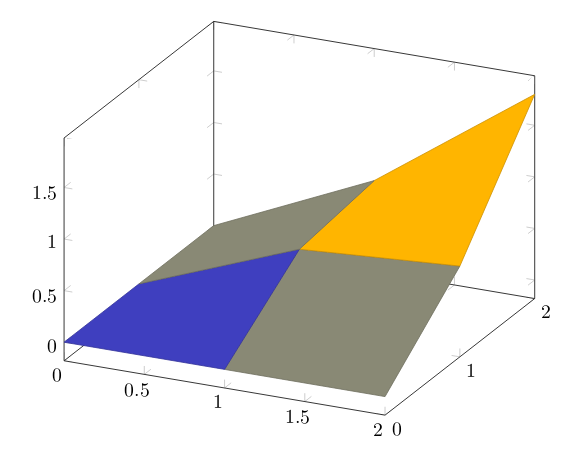
\includegraphics[width=8cm]{Pgfplot3d3}
\caption{Three dimensional graph}
\label{fig:figure1}
\end{figure}


\chapter{What I prefer}
My prefs

\chapter{Reason and Observations}
My prefs

\chapter{Applications}

\section{Applications in general}
Here we will look at two types of applications for our proposed work. One is outcome of its generacity and another is due to the specific focus of the objectives for this work. When we talk about general applications, following are the most obvious ones and
have been prevalently the raison-de-etre for this research.
\begin{itemize*}
  \item \textbf{Spam Filtering} a process which tries to discern E-mail spam messages from legitimate emails
  \item \textbf{Email Routing} sending an email sent to a general address to a specific address or mailbox depending on topic
  \item \textbf{Language Identification} automatically determining the language of a text
  \item \textbf{genre classification} automatically determining the genre of a text (also the objective of this work)
  \item \textbf{readability assessment} automatically determining the degree of readability of a text, either to find suitable materials for different age groups or reader types or as part of a larger text simplification system 
  \item \textbf{sentiment analysis} determining the attitude of a speaker or a writer with respect to some topic or the overall contextual polarity of a document.
  \item \textbf{Article triage} selecting articles that are relevant for manual literature curation, for example as is being done as the first step to generate manually curated annotation databases in biology.
\end{itemize*}

\section{Application in Ecommerce (Purpose of this work)}
Here we will talk about the prime motivator for this work. 


\chapter{Conclusions}
Applications

\begin{thebibliography}{12}
	\bibitem{wikipedia-textclassification}
	  Wikipedia,
	  \emph {http://en.wikipedia.org/wiki/Document\_classification}.
	\bibitem{paper-atctechreview}
	  Automatic Text Classification,
	  Internation Journal of Computer Applications (0975 - 8888)
	  Volume 28 - No. 2, August 2011
	\bibitem{paper-ann-svm}
	  Online News Text Classification Using Neural Network and SVM,
	  Raghvan Gachli, International Journal of Latest Scientific Research and Technology 1(2), July - 2014, pp. 122-128, ISSN: 2348-9464
	\bibitem{paper-product-cat}
	  Applying Machine Learning to Product Categorization,
	  Sushant Shankar and Irving Lin,
	  Department of Computer Science, Standford University.
	\bibitem{paper-semantic-kernels}
	  Building Semantic Kernels for Text Classification using Wikipedia,
	  Pu Wang and Carlotta Domeniconi,
	  Department of Computer Science, George Mason University.
	\bibitem{paper-goldenbullet}
	  GoldenBullet: Automated Classification of Product Data in E-Commerce,
	  Y. Ding, M. Korotkiy, B. Omelayenko, V. Kartseva, V. Zykov, M. Klien, E. Schulten and D. Fensel.
	  Vrije Universiteit Amsterdam, De Boelelaan 1081a, 1081 HV Amsterdam, NL.
\end{thebibliography} %Must end the environment


\end{document}  %End of document.
